% Template for a Computer Science Tripos Part II project dissertation
\documentclass[12pt,a4paper,twoside,openright]{report}
\usepackage[pdfborder={0 0 0}]{hyperref}    % turns references into hyperlinks
\usepackage[margin=25mm]{geometry}  % adjusts page layout
\usepackage{graphicx}  % allows inclusion of PDF, PNG and JPG images
\usepackage{verbatim}
\usepackage{docmute}   % only needed to allow inclusion of proposal.tex

\raggedbottom                           % try to avoid widows and orphans
\sloppy
\clubpenalty1000%
\widowpenalty1000%

\renewcommand{\baselinestretch}{1.1}    % adjust line spacing to make
                                        % more readable

\begin{document}

\bibliographystyle{plain}


%%%%%%%%%%%%%%%%%%%%%%%%%%%%%%%%%%%%%%%%%%%%%%%%%%%%%%%%%%%%%%%%%%%%%%%%
% Title


\pagestyle{empty}

\rightline{\LARGE \textbf{George Ash}}

\vspace*{60mm}
\begin{center}
\Huge
\textbf{} \\[5mm]
Computer Science Tripos -- Part II \\[5mm]
Fitzwilliam College \\[5mm]
\today  % today's date
\end{center}

%%%%%%%%%%%%%%%%%%%%%%%%%%%%%%%%%%%%%%%%%%%%%%%%%%%%%%%%%%%%%%%%%%%%%%%%%%%%%%
% Proforma, table of contents and list of figures

\pagestyle{plain}

\chapter*{Proforma}

{\large
\begin{tabular}{ll}
Name:               & \bf George Ash                       \\
College:            & \bf Fitzwilliam College                     \\
Project Title:      & \bf Smart Antialiasing for Consumer Virtual Reality \\
Examination:        & \bf Computer Science Tripos -- Part II, July 2017  \\
Word Count:         & \bf 1587\footnotemark[1]
                      (well less than the 12000 limit)  \\
Supervisor:         & Dr Rafal Mantiuk                    \\ 
\end{tabular}
}
\footnotetext[1]{This word count was computed
by \texttt{detex diss.tex | tr -cd '0-9A-Za-z $\tt\backslash$n' | wc -w}
}
\stepcounter{footnote}


\section*{Original Aims of the Project}



\section*{Work Completed}

All that has been completed appears in this dissertation.

\section*{Special Difficulties}

Learning how to incorporate encapulated postscript into a \LaTeX\
document on both Ubuntu Linux and OS X.
 
\newpage
\section*{Declaration}

I, [Name] of [College], being a candidate for Part II of the Computer
Science Tripos [or the Diploma in Computer Science], hereby declare
that this dissertation and the work described in it are my own work,
unaided except as may be specified below, and that the dissertation
does not contain material that has already been used to any substantial
extent for a comparable purpose.

\bigskip
\leftline{Signed [signature]}

\medskip
\leftline{Date [date]}

\tableofcontents

\listoffigures

\newpage
\section*{Acknowledgements}

This document owes much to an earlier version written by Simon Moore
\cite{Moore95}.  His help, encouragement and advice was greatly 
appreciated.

%%%%%%%%%%%%%%%%%%%%%%%%%%%%%%%%%%%%%%%%%%%%%%%%%%%%%%%%%%%%%%%%%%%%%%%
% now for the chapters

\pagestyle{headings}

\chapter{Introduction}

\section{Overview of the files}

This document consists of the following files:

\begin{itemize}
\item \texttt{makefile} --- The makefile for the dissertation and
                         Project Proposal
\item \texttt{diss.tex} --- The dissertation
\item \texttt{proposal.tex}  --- The project proposal 
\item \texttt{figs} -- A directory containing diagrams and pictures
\item \texttt{refs.bib} --- The bibliography database
\end{itemize}

\section{Building the document}

This document was produced using \LaTeXe which is based upon
\LaTeX\cite{Lamport86}.  To build the document you first need to
generate \texttt{diss.aux} which, amongst other things, contains the
references used.  This if done by executing the command:

\texttt{pdflatex diss}

\noindent
Then the bibliography can be generated from \texttt{refs.bib} using:

\texttt{bibtex diss}

\noindent
Finally, to ensure all the page numbering is correct run \texttt{pdflatex}
on \texttt{diss.tex} until the \texttt{.aux} files do not change.  This
usually takes 2 more runs.

\subsection{The OpenGL pipeline}

The OpenGL pipeline is comprised of several stages. As graphics programmers we generally only concern ourselves with two of the programmable stages: The fragment shader and the vertex shader.

From the vertex shaders perspective, it is provided with an individual vertex, and the data that might be associated with it (3d Cartesian coordinates, Vertex Colour, UV Texture coordinates) These are then processed arbitrarily by the vertex shader. And passed onto vertex Post-Processing stage, which we have little or no control over as programmers.

From the fragment shaders perspective, we are provided implicitly with our fragments position within the viewport (Including depth information) and any other data that was passed on by the vertex shader (Texture coordinates). We can then perform lighting calculations, texture lookups in this stage.

\begin{description}

\item\texttt{make} \\
 Display help information.

\item\texttt{make proposal.pdf} \\
 Format the proposal document as a PDF.

\item\texttt{make view-proposal} \\
 Run \texttt{make proposal.pdf} and then display it with a Linux PDF viewer
 (preferably ``okular'', if that is not available fall back to ``evince'').

\item\texttt{make diss.pdf} \\
 Format the dissertation document as a PDF.

\item\texttt{make count} \\
Display an estimate of the word count.

\item\texttt{make all} \\
Construct \texttt{proposal.pdf} and \texttt{diss.pdf}.

\item\texttt{make pub} \\ Make \texttt{diss.pdf}
and place it in my \texttt{public\_html} directory.

\item\texttt{make clean} \\ Delete all intermediate files except the
source files and the resulting PDFs. All these deleted files can
be reconstructed by typing \texttt{make all}.

\end{description}


\section{Anti-Aliasing techniques}

Aliasing occurs when we misrepresent a signal frequency as we sample it. 
To ameliorate artefacts such as these in a graphics pipeline we can employ one of various techniques:

\subsection{Multisample Anti-aliasing}

The default technique employed by OpenGL, this technique samples a number of times only along polygon edges and downsamples the fragment before it is passed to the fragment shader. In most scenarious this approach is adequate, but this technique fails where artefacts are visible inside of polygons boundaries.

\subsection{Supersample Anti-aliasing}

Being the simplest approach, we take multiple samples for each pixel onscreen, and downsample before presenting the image.

This approach h results in the best image, and can ameliorate aliasing inside of polygon boundaries.
\texttt{wc diss.tex}

\noindent
Alternatively, try something like:

\verb/detex diss.tex | tr -cd '0-9A-Z a-z\n' | wc -w/


\chapter{Preparation}

This chapter is empty!


\chapter{Implementation}

\section{Verbatim text}

Verbatim text can be included using \verb|\begin{verbatim}| and
\verb|\end{verbatim}|. I normally use a slightly smaller font and
often squeeze the lines a little closer together, as in:

{\renewcommand{\baselinestretch}{0.8}\small
\begin{verbatim}
GET "libhdr"
 
GLOBAL { count:200; all  }
 
LET try(ld, row, rd) BE TEST row=all
                        THEN count := count + 1
                        ELSE { LET poss = all & ~(ld | row | rd)
                               UNTIL poss=0 DO
                               { LET p = poss & -poss
                                 poss := poss - p
                                 try(ld+p << 1, row+p, rd+p >> 1)
                               }
                             }
LET start() = VALOF
{ all := 1
  FOR i = 1 TO 12 DO
  { count := 0
    try(0, 0, 0)
    writef("Number of solutions to %i2-queens is %i5*n", i, count)
    all := 2*all + 1
  }
  RESULTIS 0
}
\end{verbatim}
}

\section{Tables}

\begin{samepage}
Here is a simple example\footnote{A footnote} of a table.

\begin{center}
\begin{tabular}{l|c|r}
Left      & Centred & Right \\
Justified &         & Justified \\[3mm]
%\hline\\%[-2mm]
First     & A       & XXX \\
Second    & AA      & XX  \\
Last      & AAA     & X   \\
\end{tabular}
\end{center}

\noindent
There is another example table in the proforma.
\end{samepage}

\section{Simple diagrams}

Simple diagrams can be written directly in \LaTeX.  For example, see
figure~\ref{latexpic1} on page~\pageref{latexpic1} and see
figure~\ref{latexpic2} on page~\pageref{latexpic2}.

\begin{figure}
\setlength{\unitlength}{1mm}
\begin{center}
\begin{picture}(125,100)
\put(0,80){\framebox(50,10){AAA}}
\put(0,60){\framebox(50,10){BBB}}
\put(0,40){\framebox(50,10){CCC}}
\put(0,20){\framebox(50,10){DDD}}
\put(0,00){\framebox(50,10){EEE}}

\put(75,80){\framebox(50,10){XXX}}
\put(75,60){\framebox(50,10){YYY}}
\put(75,40){\framebox(50,10){ZZZ}}

\put(25,80){\vector(0,-1){10}}
\put(25,60){\vector(0,-1){10}}
\put(25,50){\vector(0,1){10}}
\put(25,40){\vector(0,-1){10}}
\put(25,20){\vector(0,-1){10}}

\put(100,80){\vector(0,-1){10}}
\put(100,70){\vector(0,1){10}}
\put(100,60){\vector(0,-1){10}}
\put(100,50){\vector(0,1){10}}

\put(50,65){\vector(1,0){25}}
\put(75,65){\vector(-1,0){25}}
\end{picture}
\end{center}
\caption{A picture composed of boxes and vectors.}
\label{latexpic1}
\end{figure}

\begin{figure}
\setlength{\unitlength}{1mm}
\begin{center}

\begin{picture}(100,70)
\put(47,65){\circle{10}}
\put(45,64){abc}

\put(37,45){\circle{10}}
\put(37,51){\line(1,1){7}}
\put(35,44){def}

\put(57,25){\circle{10}}
\put(57,31){\line(-1,3){9}}
\put(57,31){\line(-3,2){15}}
\put(55,24){ghi}

\put(32,0){\framebox(10,10){A}}
\put(52,0){\framebox(10,10){B}}
\put(37,12){\line(0,1){26}}
\put(37,12){\line(2,1){15}}
\put(57,12){\line(0,2){6}}
\end{picture}

\end{center}
\caption{A diagram composed of circles, lines and boxes.}
\label{latexpic2}
\end{figure}



\section{Adding more complicated graphics}

The use of \LaTeX\ format can be tedious and it is often better to use
encapsulated postscript (EPS) or PDF to represent complicated graphics.
Figure~\ref{epsfig} and~\ref{xfig} on page \pageref{xfig} are
examples. The second figure was drawn using \texttt{xfig} and exported in
{\tt.eps} format. This is my recommended way of drawing all diagrams.


\begin{figure}[tbh]
\centerline{
\includegraphics{figs/cuarms.pdf}}
\caption{Example figure using encapsulated postscript}
\label{epsfig}
\end{figure}

\begin{figure}[tbh]
\vspace{4in}
\caption{Example figure where a picture can be pasted in}
\label{pastedfig}
\end{figure}


\begin{figure}[tbh]
\centerline{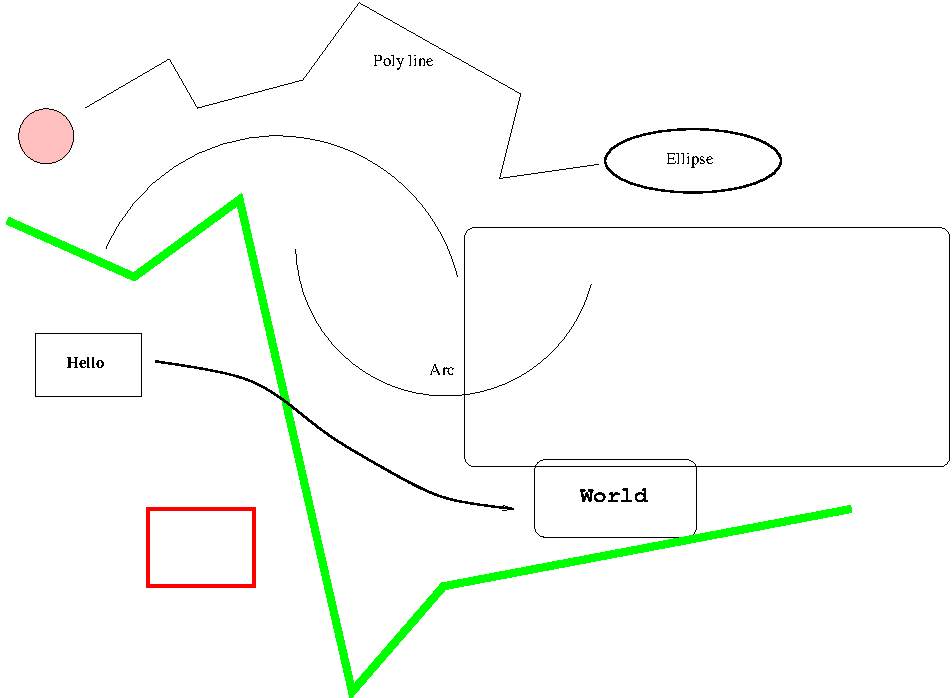
\includegraphics{figs/diagram.pdf}}
\caption{Example diagram drawn using \texttt{xfig}}
\label{xfig}
\end{figure}


\chapter{Evaluation}

\section{Optimisation}
While the approach outlined can give a unnoticably similar image to the user, it will have been for nothing if we can't perform it as quickly or slower than the default MSAA method. 

We can do a few things to speed things up:
	Decrease resolution at the edges,
	Downgrade lighting and texture calculations at the edges,
	Perform an early depth pass to exploit hardware specific early depth optimisations,
	
By far the most obvious performance improvement we can make is to run fragment shaders on fragments we know will be visible,

We render our scene twice, yet we run fragment shader code into an area of the viewport that will be overwritten my a multisampled area.

Our fragment shaders shouldn't run in these areas, so we should fail fast in areas that will be overwritten.

This snippet can be used to quickly determine if our fragment is in an area that will be overwritten.

code
code 
code

Then we only perform the useful bulk of the fragment shader code exactly the same number of times as when we weren't multisampling at all.

Alternatively we could run our render pipeline for the multisampled central area first. Then, since our depth buffer will be populated, force early depth tests on our next render pass so that fragment shaders only run on the outer edges of the image.
Because this approach doesn't run the boundary check above, we should expect better performance from this, but this early depth test optimisation is implementation specific - we can't guarantee that the approach will work on all platforms. So we don't use this optimisation.

	
\section{Further information}

See the Unix Tools notes at

\url{http://www.cl.cam.ac.uk/teaching/current-1/UnixTools/materials.html}


\chapter{Conclusion}

I hope that this rough guide to writing a dissertation is \LaTeX\ has
been helpful and saved you time.


%%%%%%%%%%%%%%%%%%%%%%%%%%%%%%%%%%%%%%%%%%%%%%%%%%%%%%%%%%%%%%%%%%%%%
% the bibliography
\addcontentsline{toc}{chapter}{Bibliography}
\bibliography{refs}

%%%%%%%%%%%%%%%%%%%%%%%%%%%%%%%%%%%%%%%%%%%%%%%%%%%%%%%%%%%%%%%%%%%%%
% the appendices
\appendix

\chapter{Latex source}

\section{diss.tex}
{\scriptsize\verbatiminput{diss.tex}}

\section{proposal.tex}
{\scriptsize\verbatiminput{proposal.tex}}

\chapter{Makefile}

\section{makefile}\label{makefile}
{\scriptsize\verbatiminput{makefile.txt}}

\section{refs.bib}
{\scriptsize\verbatiminput{refs.bib}}


\chapter{Project Proposal}

% Note: this file can be compiled on its own, but is also included by
% diss.tex (using the docmute.sty package to ignore the preamble)
\documentclass[12pt,a4paper,twoside]{article}
\usepackage[pdfborder={0 0 0}]{hyperref}
\usepackage[margin=25mm]{geometry}
\usepackage{graphicx}
\usepackage{parskip}
\begin{document}

\begin{center}
\Large
Computer Science Tripos -- Part II -- Project Proposal\\[4mm]
\LARGE
Smart Anti-Aliasing for Virtual Reality \\[4mm]

\large
G.~Ash, Fitzwilliam College

12 October 2016
\end{center}

\vspace{5mm}

\textbf{Project Supervisor:} Dr R.~Mantiuk

\textbf{Director of Studies:} Dr R.~Harle

\textbf{Project Overseers:} Prof R.~Anderson  \& Prof J.~Bacon

% Main document

\section*{Introduction}

A problem with modern Virtual Reality headsets is that they use low resolution displays to cover a huge Field of View.
Graphical artefacts, such as moir\'e patterns and pixellated edges (jaggies), are pronounced on these displays.
A good technique to ameliorate these artefacts if super-sampling, but super-sampling is often too expensive in VR
devices where low latency is a requirement - to avoid simulation sickness. 

Unfortunately, modern consumer headsets suffer from astigmatism because of a single lens between the viewer and the display. We can't remove these distortions without (another) anastigmatic lens, however we do currently give equal preference to image quality across the whole of the display even when the edges of the image become distorted.

\begin{figure}[tbh]
\centerline{
\includegraphics[width=0.3\linewidth]{figs/blur.png}}
\caption{The center of the perceived image is sharp, while the edges get progressively blurrier}
\label{blurfig}
\end{figure}

We could exploit astigmatism in single lens VR headsets by sampling more in the sharp center of the image,
and sampling less as we move towards the blurrier edges (Figure \ref{blurfig}). This project aims to extend an existing open source system to include this optimisation, and to measure the impact on both the performance of the system, and on the image quality to the user.

\section*{Starting point}

Novel anti-aliasing techniques, such as subpixel-reconstruction and temporal antialiasing, are still actively being developed. I intend to build on Intel's research[1] into a hybrid raytracing/rasterizing VR renderer by creating an entirely rasterized solution that retains image quality while allowing for GPU hardware acceleration.

Free and extensible renderers exist for VR headsets, such as Unity. However I will be extending the existing open-source OSVR-RenderManager, which will allow me to easily create separate reusable demos to show off certain graphical artefacts, and, if neccesary, to modify the entire rendering pipeline.
OSVR is compatible with all modern VR headsets, and supports all modern graphics APIs (OpenGL, Vulkan, Direct3D).

I have good experience in C/C++ through small projects and the IB C/C++ course. I'm familiar with the graphics pipeline and have experience in WebGL, with some experience writing vertex and fragment shaders in OpenGL. I will need to refresh my knowledge of shader programming, and will need to take some time learning most of the OpenGL API.

\section*{Resources required}

For this project I shall be using my own quad-core machine with a VR capable GPU. I will also be using an Occulus Rift Development Kit 2 [3](lent to me by the Hackers at Cambridge group) for testing and user studies. Source backups will be made both to a private Github repository and MCS daily.
I will use an MCS machine as a failsafe incase my machine should break.

\section*{Work to be done}

The project breaks down into the following sub-projects:

\begin{enumerate}

\item \textbf{Setup} Fork the existing Open Source Virtual Reality-RenderManager repository. Create a daily cronjob to backup this to github and MCS. Research my chosen renderer's pipeline.

\item \textbf {Core development} Develop/modify a simple super-sampling algorithm. Extend the algorithm to allow for areas of the screen to be ignored. Further extend to seamlessly composite draws that we sample differently.

\item \textbf {Demo creation} Create a couple of OpenGL demos that highlight both moire patterns and pixellated edges, for use in visual quality experiment.

\item \textbf {Optimisation} Make use of a GPU profiler to determine any redundancy or inefficiency. Refactor the algorithm to make it easily configurable.

\item \textbf {Evaluation} Make use of benchmarking/profiling software to evaluate the algorithm with regards to performance. Perform visual quality experiment to evaluate the impact of the algorithm on image quality to the user, recruit college members across fields to participate. Compare my approach against no anti-aliasing, and fullscreen anti-aliasing.

\end{enumerate}

\section*{Success citeria}

The project will be a success if I manage to do the following:
\begin{enumerate}

\item Improve the performance of the open source renderer with anti-aliasing enabled

\item Provide an alternative anti-aliasing technique that suffers only negligible loss in image quality to the end user.

\item Evaluate both full screen antialiasing, my selective antialiasing approach, and no antialiasing from a user perspective by constructing demos that show off artefacts masked by antialiasing.

\end{enumerate}

\section*{Possible extensions}

If I achieve my main result early I shall try the following
alternative experiment or method of evaluation:

\begin{enumerate}

\item Research using a heuristic to determine salient objects or regions in the scene, and extend my algorithm to more closely resemble a foveated rendering[2] technique.

\item Further reduce the requirement to super-sample by determining which objects/samples can be shared between each eye.

\end{enumerate}





\section*{Timetable}

Planned starting date is 16/10/2011.

\begin{enumerate}

\item \textbf{Michaelmas weeks 2--4} Start project Setup, Begin refreshing knowledge on OpenGL. Research the rendering pipeline of my chosen renderer. Formulate an implementation strategy.

\item \textbf{Michaelmas weeks 5--6} Complete project setup. Test writing custom code in the renderer, start implementation of selective antialiasing algorithm

\item \textbf{Michaelmas weeks 7--8} Continue development of algorithm. Start on demo creation

\item \textbf{Michaelmas vacation} Finish development of algorithm and demos.

\item \textbf{Lent weeks 0--2} Write progress report. Generate corpus of
  test examples. Begin optimisation.

\item \textbf{Lent weeks 3--5} Finish optimisation, begin evaluation of image quality on users.  

\item \textbf{Lent weeks 6--8} Finish user studies, start performance analysis. Write up User studies in disseration.

\item \textbf{Easter vacation:} Begin on extensions, flesh out dissertation, complete evaluation. 

\item \textbf{Easter term 0--2:}  Complete dissertation, proof read. Submit to DoS and supervisor for comments. 

\item \textbf{Easter term 3:} Further proof reading/refactoring and submit dissertation.

\end{enumerate}

\section*{References}

\begin{enumerate}

\item Using Astigmatism in Wide Angle HMDs to Improve Rendering D. Pohl, T. Bolkart, S. Nickels, O. Grau, 2015.
\item Foveated 3d graphics. B. Guenter, M. Finch, S. Drucker, D. Tan, and J. Snyder. ACM SIGGRAPH Asia, 2012.
\item Oculus VR. Oculus Rift, 2014. http://www.oculus.com/

\end{enumerate}

\end{document}


\end{document}
